\section{\tool}
\label{sec:badusb}
\subsection{Threat Model}
We build our threat model on the basic assumptions that common users without technical background would not treat normal-looking USB device as highly dangerous and be cautious about them. These assumptions are approved in a relevant work about charging attack\cite{JFCImpact}. Moreover, we neglect the effect of notification about common USB device, as normal users usually are not equipped with the necessary knowledge to fully understand such notices. In fact, during our experiment, no device had security notifications raised about suspicious USB devices and only mobile devices had raised charging notification about our \tool, which is not a sufficient warning towards users.

We also assume the victim's device is equipped with fully functional USB 3.x protocol and USB Type C connector. As the USB 3.x standard is more and more common around the world, this assumption can be easily fulfilled especially in recent devices.
\subsection{Motivation}
\noindent\outline{Limitation of Rubber Ducky}\\
\outline{Our functionality different mode listing?}\\
\hongyi{The following mode is to be further decided}
\outline{Automatic Scripting Mode}\\
\outline{Remote Control Mode}\\
\outline{OCR/QR Recognition Mode}\\
As we introduced in the Section~\ref{sec:related_work}, there are plenty of existing work \shuqing{Add citation} focusing on BadUSB attack. 
Many of these take advantage of the \textit{trust-by-default} policy of PC, pretend normal HID devices and utilize USB protocol to perform attacks. 
However, these attacks suffer from various drawbacks:
\ding{182} attackers can only simulate limited types of devices such as HIDs (like keyboards and mice) and disks, which makes the attacks less effective;
\ding{183} accurate attacks couldn't be performed due to lack of user interface (UI).
Whatever HID the attackers simulate their USB devices to be, they couldn't obtain the UI to check the current situation, which makes it nearly impossible to locate their attacks precisely or confirm the effects after attacks.

In this work, we utilized the new features of USB 3.x \cite{usb31} \cite{usb32} to address the problems above.
Benefiting from latest protocol, we simulated video card and thus obtained the video stream to perform accurate attacks.

\subsection{Implementation}
\noindent\hongyi{The following mode is to be further decided}\\
\outline{DETAIL of each mode}\\
\outline{Automatic Scripting Mode}\\
\outline{Remote Control Mode}\\
\outline{OCR/QR Recognition Mode}\\
Though Rubber Ducky\cite{rubber} emulates as a HID device enabling various arbitrary execution attacks, fetching feedback from the victim is much more limited. Based on this restriction several defense mechanisms were proposed  like GoodUSB\cite{tian2015defending}\hongyi{We need more example}. These defense mechanism implemented a CAPTCHA-like\cite{captcha} procedure, which requires user to complete certain challenges when a unknown HID device is plugged in. As the Rubber Ducky is only able to emulate HID device, by no means the Rubber Ducky can bypass it. Our \tool, on the other hand, is capable of bypassing this type of defense. Taking advantage of USB 3.x\cite{usb31}\cite{usb32}, \tool can fetch the video stream of the victim and complete the challenge automatically or manually. Moreover, with video capability, our \tool achieved multiple new threat model and are tested under various scenarios.

As there were various Rubber Ducky implementation available, we only focus on its core functionality and our extension. In this section, we first introduce the hardware components we used to build \tool, then we focus on the three different attack modes we implement  for various scenario.

\subsubsection{Attack Model}
The components in our attack model are as follows and the relation between them is illustrated at Fig.~\ref{fig:attack_model}
\begin{itemize}
	\item\textit{USB 3.x Hub} exports the USB 3.x connector into various ports, like DisplayPort, USB 2.0 port etc.
	\item\textit{Video Capture Card} convert DisplayPort signal into UVC-compatible\hongyi{citation needed} data, which is later processed by Raspberry Pi.
	\item\textit{Single Board Computer} processes video stream from the victim where private data is extracted and transmitted through GSM/WiFi.
	\item\textit{HID Emulator} emulates HID device which can be controlled from either the embedded Raspberry Pi or the attacker.
\end{itemize}
\begin{figure}[hbtp]
	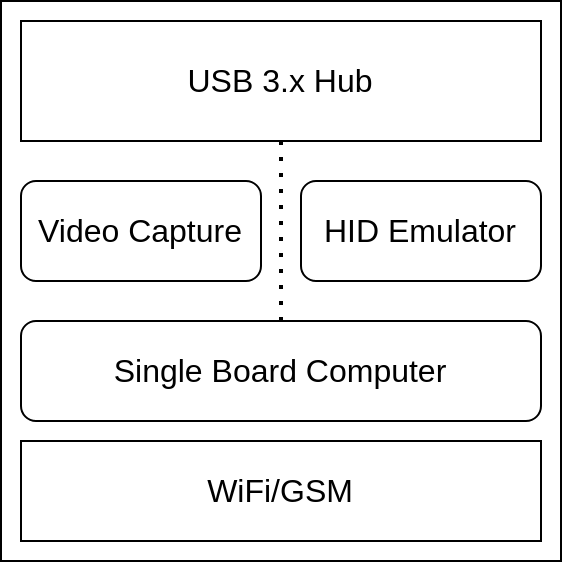
\includegraphics[width=\linewidth]{./Figs/attack_model.png}
	\caption{Attack Model}
	\label{fig:attack_model}
\end{figure}
\textbf{Scripting Mode}
\tool under this mode works almost the same like the original Rubber Ducky with various improvement.

First \tool supports defense mechanism bypass. As the original Rubber Ducky cannot get feedback from the victim, defense mechanism like GoodUSB \cite{tian2015defending} is sufficient to prevent these BadUSB attack. But such defense mechanism needs visual notification to request authentication for unknown USB device. This means that when the defense request authentication from the user, our \tool is able to capture the content of authentication challenge and complete it automatically or manually. After the defense is bypassed, \tool continues the emulation and script execution, resulting a successful attack.

As the mouse relies on the visual feedback to work properly, its emulation and automation were not supported by the original version of Rubber Ducky. Yet with the video output support from USB 3.x, our \tool implements full-functional mouse emulation. This function enables attacks toward pure GUI programs and showed great potential in mobile attack scenario. Details can be obtained in Section~\ref{sec:experiment}.

The advantage of this mode is that it archives defense bypass and attack feedback with low overhead. As mentioned above, we only require video stream at the begin(defense bypass) and the end(feedback) of the attack. Moreover, with mouse supported, \tool extends the original BadUSB attack surface and perform well in mobile device.

\textbf{Remote Control Mode}
In \tool, we implement all components required to operate a computer/mobile remotely, including a video stream, keyboard/mouse emulation.

\tool under this mode follows a simple logic. \tool will receive video stream from the victim's device and redirect it to the attacker via GSM/WiFi. In the meanwhile, \tool also receives commands from the attacker through GSM/WiFi and replay them to the victim by USB emulation.

This mode enable attacker to perform delicate operation that is beyond automation. Moreover, this mode provides a backdoor that does not require host network and thus is undetectable by firewall running on the host machine.
\hongyi{I think this is a quite good selling point?}\shuqing{Agree with Hongyi.}

The advantage of this mode is that it can completely hijack the victim device. But this complete control also comes with the price of high power consumption and risk of being detected by the user.

\textbf{Privacy Extraction Mode}
\tool under this mode does not emulate other USB device and solely rely on the video stream function of USB 3.x.

When running in this mode, \tool passively process the victim's video stream and detect for ``valuable'' private data.  Here, a data is ``valuable'' or not is decided by a customized detector, we implement a simple one of payment code for demonstration purpose. Though this detector is simple to implement, we successfully transfer money from the victim. More detail can be obtained in Section~\ref{sec:experiment}.

It is worth mentioning that \tool under this mode is completely passive, making it hard to be detected and defended. With different detector implemented, \tool under this mode is capable of serving more purpose.

Though \tool under this mode is least detectable, \tool is also unable to fetch any information actively. All the video stream has to be analyzed and filtered to become usable private information.
